\documentclass[conference]{IEEEtran}
%\IEEEoverridecommandlockouts
% The preceding line is only needed to identify funding in the first footnote. If that is unneeded, please comment it out.
\usepackage{cite}
\usepackage{amsmath,amssymb,amsfonts}
\usepackage{algorithmic}
\usepackage{graphicx}
\usepackage{textcomp}
\usepackage{xcolor}
\def\BibTeX{{\rm B\kern-.05em{\sc i\kern-.025em b}\kern-.08em
    T\kern-.1667em\lower.7ex\hbox{E}\kern-.125emX}}
\begin{document}

\title{Epidemic Simulator\\}

% figure sample
%\begin{figure}[!t]
%\centering
%\includegraphics[width=2.5in]{myfigure}
%\caption{Simulation results for the network.}

\author{\IEEEauthorblockN{Mathew Reilly}
\IEEEauthorblockA{\textit{Undergrad, Dept. Computer Science} \\
\textit{University of Central Florida}\\
Orlando FL, USA \\
ma288914@ucf.edu}
\and
\IEEEauthorblockN{Anthony Cobb}
\IEEEauthorblockA{\textit{Undergrad, Dept. Computer Science} \\
\textit{University of Central Florida}\\
Orlando FL, USA \\
an824794@ucf.edu}
\and
\IEEEauthorblockN{Sebastien Joseph}
\IEEEauthorblockA{\textit{Undergrad, Dept. Computer Science} \\
\textit{University of Central Florida}\\
Orlando FL, USA \\
se788033@ucf.edu}
\and
\IEEEauthorblockN{Adrian Hernandez}
\IEEEauthorblockA{\textit{Undergrad, Dept. Computer Science} \\
\textit{University of Central Florida}\\
Orlando FL, USA \\
aahernandez@ucf.edu}
\and
\IEEEauthorblockN{Tra’Von Ross}
\IEEEauthorblockA{\textit{Undergrad, Dept. Computer Science} \\
\textit{University of Central Florida}\\
Orlando FL, USA \\
tr500226@ucf.edu}
}

\maketitle

\begin{abstract}
Having a grasp on epidemic spread can be difficult to visualize. There are many factors that impact the spread of infections such as physical distance, communities, and immunity. To aid in the understanding of epidemics, we aimed to create a simulation that showcases some of this complexity while providing an easier way to visualize communities. Additionally, to help visualize large populations, we utilize multithreading to improve our simulation’s performance. Our program splits the communities into sections where threads are responsible for simulating the algorithm on that section. This improvement in performance allows larger simulations to perform better, improving the visual experience of our simulator.
\end{abstract}

\begin{IEEEkeywords}
SIR, epidemic, simulator
\end{IEEEkeywords}

\section{Introduction}
In the far past, communities were ravaged by all manner of diseases; most famously, the Black Death. Their spread seemed almost unstoppable due to a lack of effective methods of prediction and prevention. Without any way to anticipate the spread of a disease, societies were left vulnerable to their impact. As time passes, our knowledge about medicine increases drastically allowing humanity to have a means of prevention. Unfortunately, that relies on having a valid prediction of the disease to allow for proper prevention and preparedness \cite{b7}. In response to this, our team decided to develop this disease spread simulator. The purpose of this simulator is to serve as a user-friendly platform for exploring how a disease spreads within simulated populations. We hope that by making accessible visualizations it helps inform people about how infections spread and the impact they have over communities. Ours is also just one of many disease spread simulators, and we had to be selective on the features and scope of our simulation. 

\begin{figure}[!t]
\centering
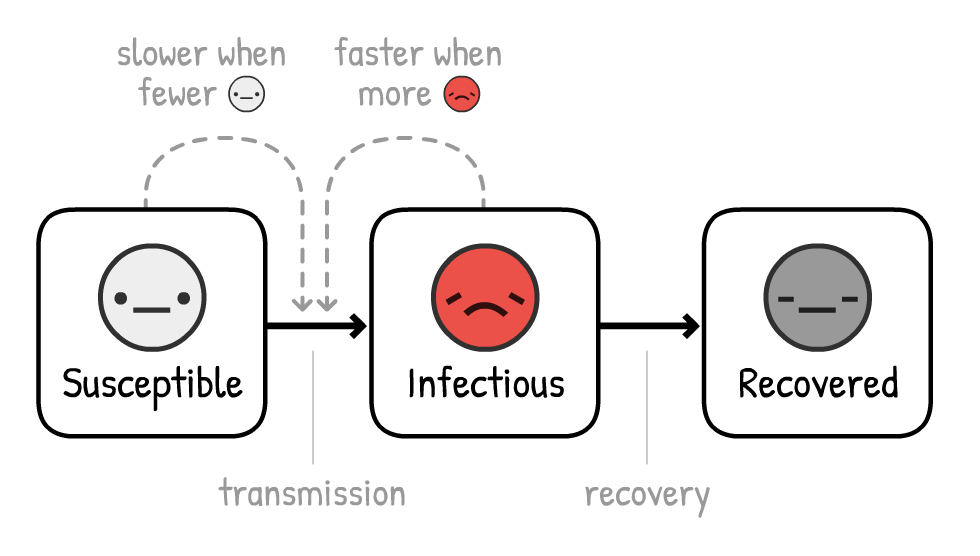
\includegraphics[width=2.5in]{Figures/ncase SIR relations.png}
\caption{Shows SIR relationships. \cite{b3}}
\label{fig_sim}
\end{figure}

We chose to focus on using a susceptible, infectious, and removed, sometimes referred to as recovered, model, commonly referred to as an SIR model, where the population could be one of these 3 states. Additionally, we wanted to model some movement patterns to create a model that gets closer to real life infectious spread. In figure 1, you see the introduction of the SIR relationships, where susceptible members can become infectious and infectious can become recovered.

\section{Problem Statement}

% \subsection{Maintaining the Integrity of the Specifications}

While there exist a myriad of other visual disease spread simulations, the majority of them lack the statistical information gathering needed to provide any actual use besides making it an appealing looking simulation. Our simulation tackles this problem by gathering statistics by leveraging the infection rates and other data obtained throughout the simulation such as the amount of infected, susceptible, and removed individuals. Our program also implements multithreading which enables faster simulation processing which in turns enables a quicker response. Using the data gathered from the simulation, proper aid and assistance can be allocated to geographical locations based on the results of the simulation. 

By focusing on implementation that collects data and is easy to visualize, we hope that our simulation can provide users with a sense of how diseases spread through communities and how far reaching sickness can be.


\section{Related Work}

As we considered how we would approach simulating an epidemic, we decided on a grid based approach. This decision was made because multiple of us were familiar with Conway's Game of Life, a population cell simulation algorithm/game. Additionally, this grid based approach has some existing implementations helping us solidify criteria we wanted for our simulation. One existing grid-based viral simulation showcases cells continually infecting each other but lacks data showcasing infection relations \cite{b1}, \cite{b2}. This gave us a good starting point for considering our implementation and multithreading questions regarding how to set up the grid. 

As we researched existing simulations we found a popular type of model, the SIR model. SIR models can be strict mathematical models showcasing how viruses get transmitted through populations \cite{b3}, or performed with a simulation visualizing the Susceptible, Infectious, and Removed, sometimes referred to as Recovered, states \cite{b4}, \cite{b5}, \cite{b6}, \cite{b8}.  An SIR model, utilizes these three possible states, representing communities and member interactions modeling infection spread. 

\subsection{Mathematical Models}

Mathematical models for SIR graphing exist and focus specifically on utilizing SIR data to create a graph. This data is not simulated through a visualization, but instead reflected through these graphs. In figure 2, the SIR graph was a composite of two common graphs, a logistic growth and a decay curve \cite{b3}. Although the combination of these graphs provides a good way to reflect data we see in the real world, it is not great at helping visualize the spread. Because of this, our model focuses more on the visualization aspect.

\begin{figure}[!hbt]
\centering
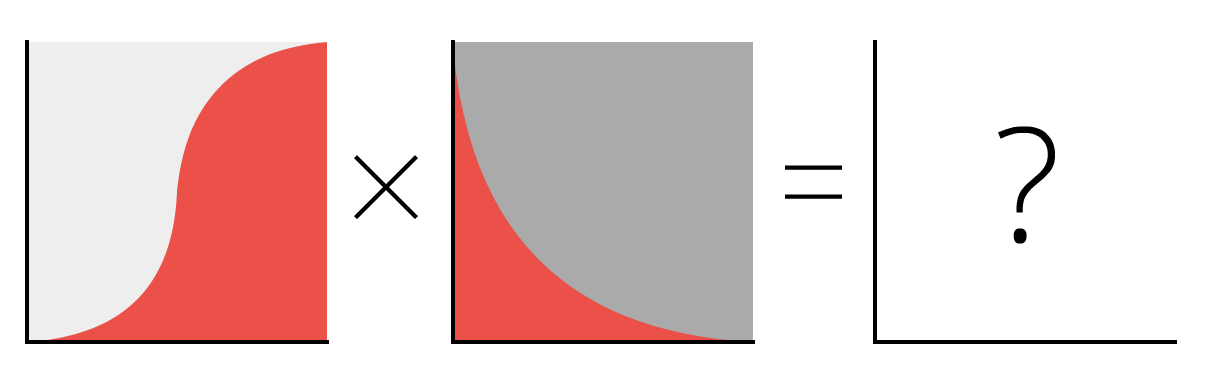
\includegraphics[width=2.5in]{Figures/SIR math Graphs - ncase .png}
\caption{Showing the two major aspects of modeling viral infections, logistic growth and decay curves \cite{b3}}
\label{fig_sim}
\end{figure}

\subsection{Visualization Modeling}

There are multiple existing visual models and simulations for infections, using the SIR model \cite{b4}, \cite{b5}, \cite{b6}, \cite{b8}. Existing implementations use different simulation techniques to represent the population and ours aims to connect some of the common themes of these existing simulations. Combining the idea of communities where cells will be traveling \cite{b4}, \cite{b6}, and a grid based approach \cite{b8}, we hoped our model would be easy for users to understand while providing more complexity than a single grid-based community. Having easy readability like figure 3 was valuable to us as it would make our simulation easy to follow.


\begin{figure}[!hbt]
\centering
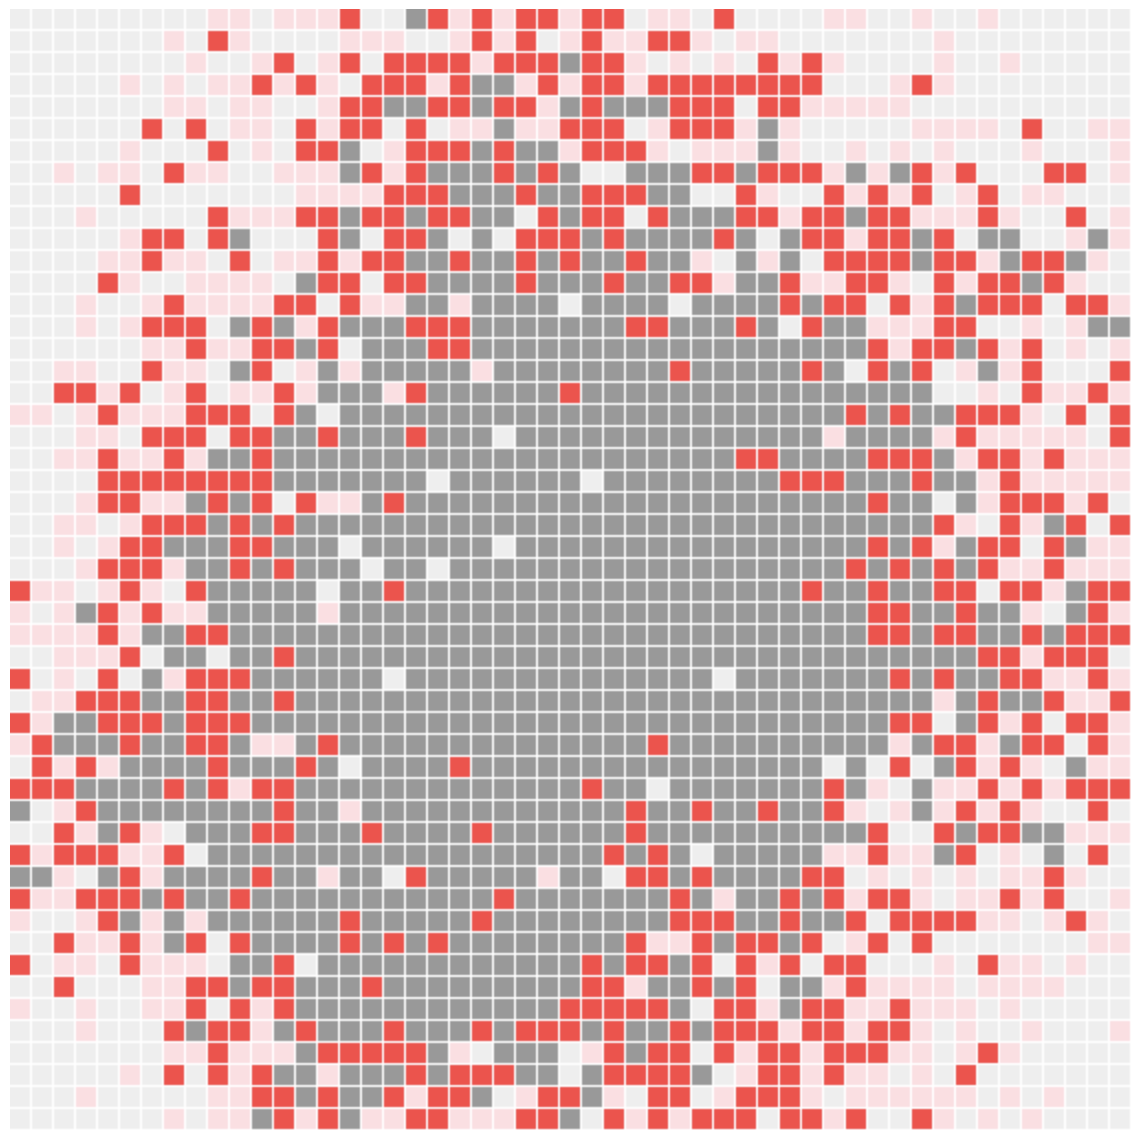
\includegraphics[width=2.5in]{Figures/Outbreak photo.png}
\caption{A simulation where cells have a travel radius representing movement \cite{b8}}
\label{fig_sim}
\end{figure}

\subsection{Our Model}

We decided that our program would relate to current simulation techniques by also using an SIR model, where each cell can be in one of these three states. Our initial testing was done with an algorithm with a similar neighboring technique to conways, where each cell would interact with its immediate neighbors and spread infections that way. Later, we progressed to implementing communities and cellular movement to be more similar to existing simulations. Although other simulations have mathematical rigor on diseases \cite{b3} we were more concerned with the visualization of the spread throughout communities.

\section{Technique}

\subsection{Multithreading}

The grid-based approach allowed for straightforward multithreading. We decided to approach multithreading by splitting the grid into sections. We split the grid into nine sections and create nine threads to handle each section of the grid. We felt that nine sections allowed for plenty of headroom for larger simulation sizes and for better performance. This method also made sure that each section would have the same amount of work to finish because each section would have the same number of cells to process, ensuring proper load balancing. 

\begin{figure}[!hbt]
\centering
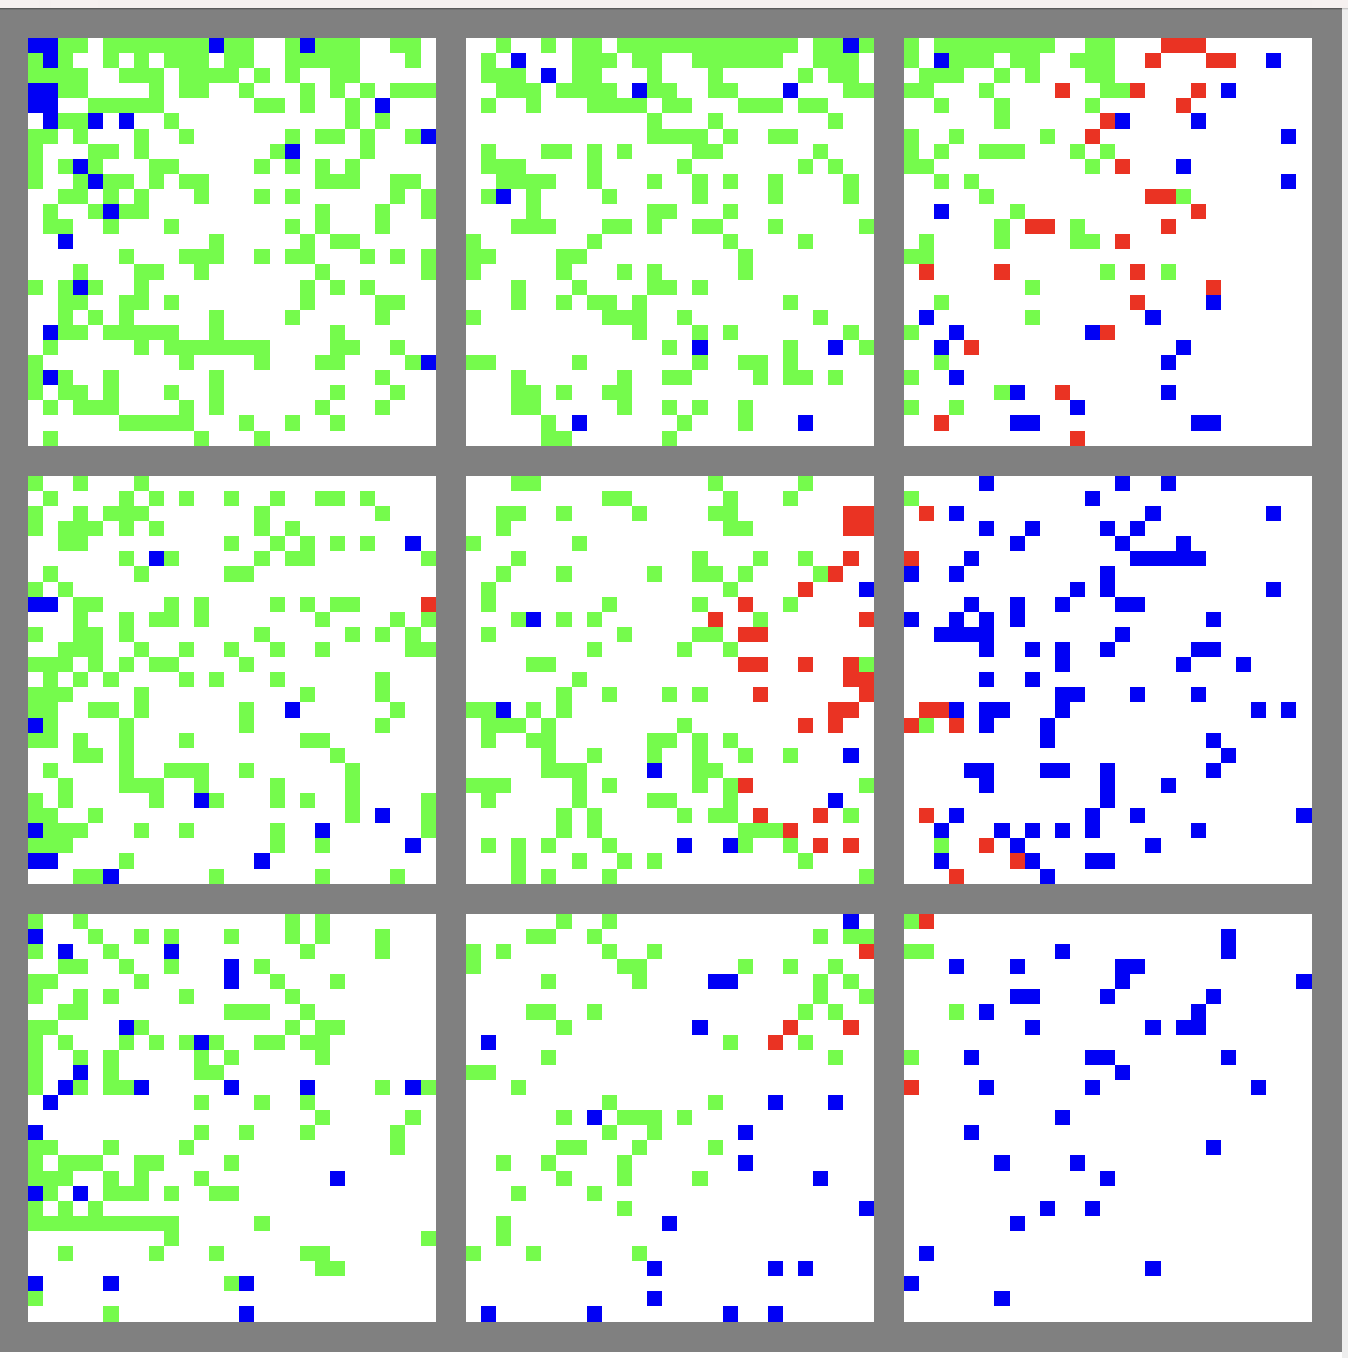
\includegraphics[width=2.5in]{Figures/Bordered Screenshot.png}
\caption{Shows borders for the cells (all 5 types can be seen) }
\label{fig_sim}
\end{figure}

To split the grid, we made padding or borders around each section which allowed for visual and practical use. We were able to easily see each section of our grid and each thread could make use of it by making sure they do not encounter any borders while processing the cells. To make sure each thread was working on the correct section, our function that controlled cell behavior, had a thread ID passed into it. The function would then determine which section of the grid it is supposed to work on based on that thread ID which then starts calculating each cell’s next state.

\begin{figure}[!hbt]
\centering
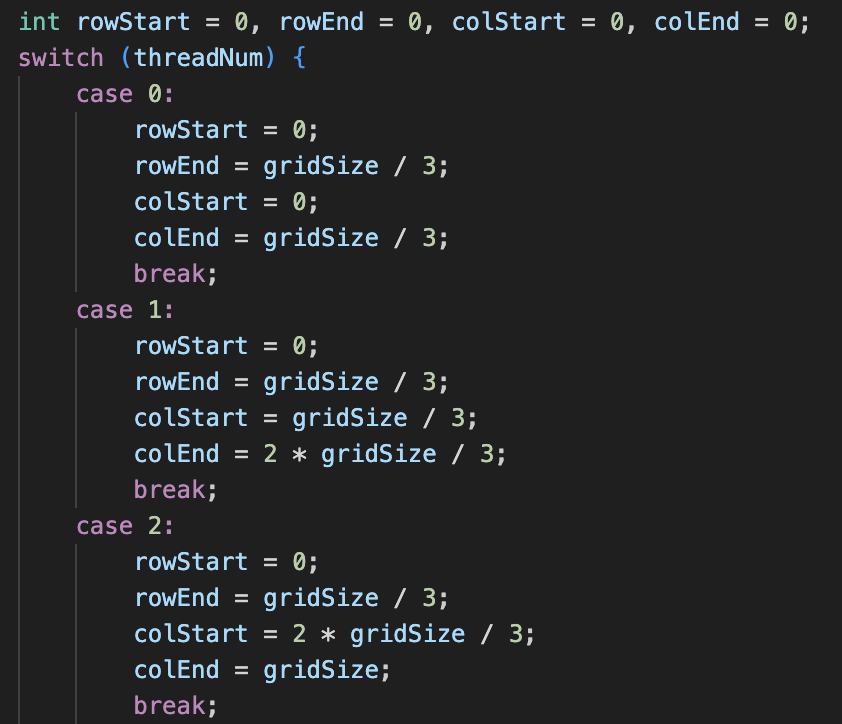
\includegraphics[width=2.5in]{Figures/multithreading divisions.png}
\caption{code that supplied thread responsibilities}
\label{fig_sim}
\end{figure}

Some limitations of this approach are that we were stuck at using nine threads so we could only test it using either one thread or all nine threads. Another limitation is that we had to make sure that the grid was a multiple of three so that the grid could evenly be split up into nine sections easily. Overall, even with this limitation, this method allowed us to have good load balancing and a simple yet effective way to multithread the simulation.

\subsection{Making Our Model Functional}

Another focus on the technique was the actual simulation steps and construction. The work that gets parallelized focuses on the infection algorithm, where based on an infection chance, the susceptible neighbors of infectious cells may also turn infected. This is split up into two parts where if a susceptible cell will be infected, it gets added to a vector first so that all newly infected cells may be processed together.

Outside of the multithreading, our program also needed to collect data on the population status, counts of the SIR, and movement to multiple communities. It was important that we included both of these aspects as we wanted our simulator to provide a more detailed model than a single community and collect the data as it is generated. The SIR data is stored in an array so that each day's data may be logged, and communities are built to all be the same size. The movement algorithm focuses on population density and has members of the population gravitate to areas that are more dense. This gathering of people will cause sections of the population to particularly vulnerable because the members are in close proximity.

\begin{figure}[!hbt]
\centering
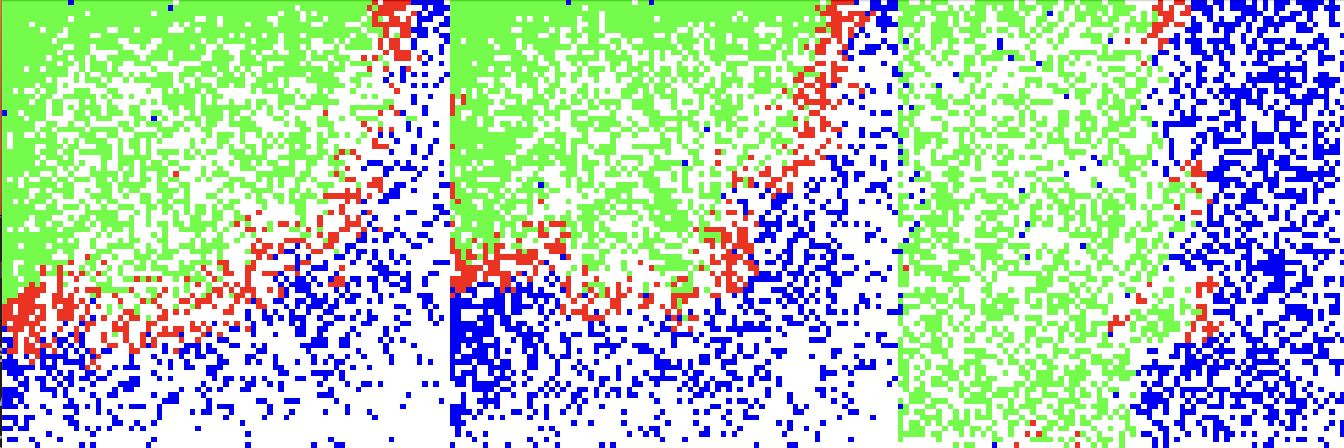
\includegraphics[width=2.5in]{Figures/multiCommunity.png}
\caption{Showing multiple community simulation, where the communities interact with each other}
\label{fig_sim}
\end{figure}

Continuing on with our implementation, we also needed to actual render our grid to visualize the simulation. Each cell is represented by a square with a color. Each color represents a state that the cell can be in. Susceptible is blue, infectious is red, and removed is green. Alternatively, instead of rendering the grid, there is an option to view a graph of how many cells are infected throughout the entire simulation. This allows us to see if our simulation matches up with other similar simulation programs. Additionally, there are several buttons and text fields that allow you to modify the size of the grid and how fast the simulation runs. This is helpful for seeing different scenarios and debugging.

\section{Evaluation}

\subsection{SIR Evaluation}

There are many ways to analyze the SIR data. Based on the independent variables, total population, starting infected population, removal rate, and infection rate, one of the metrics we chose to consider was the epidemic length. Measured in days, this starts from when the first infection appears all the way until infection reaches zero. Our model tracks multiple epidemics and determines the longest, shortest, and average epidemic length of the virus. This is useful to know, because it would let people know how long to quarantine, or how long the epidemic may last if things get out of hand.

\begin{figure}[!hbt]
\centering
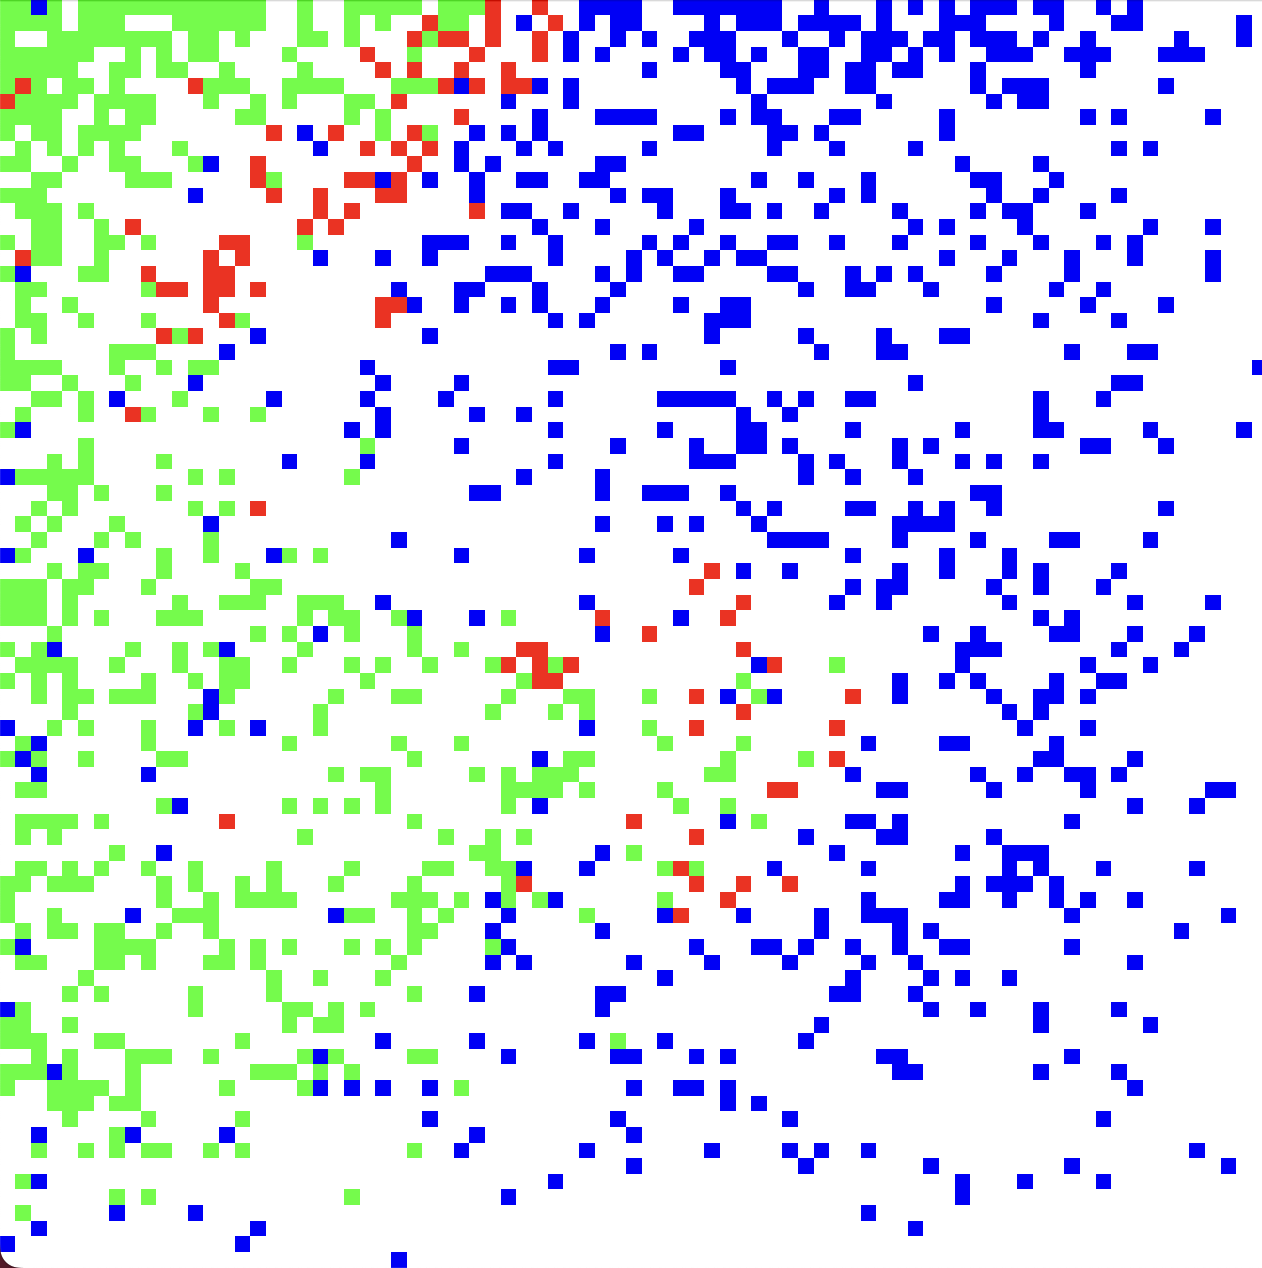
\includegraphics[width=1.25in]{Figures/Single Community Simulation Photo.png}
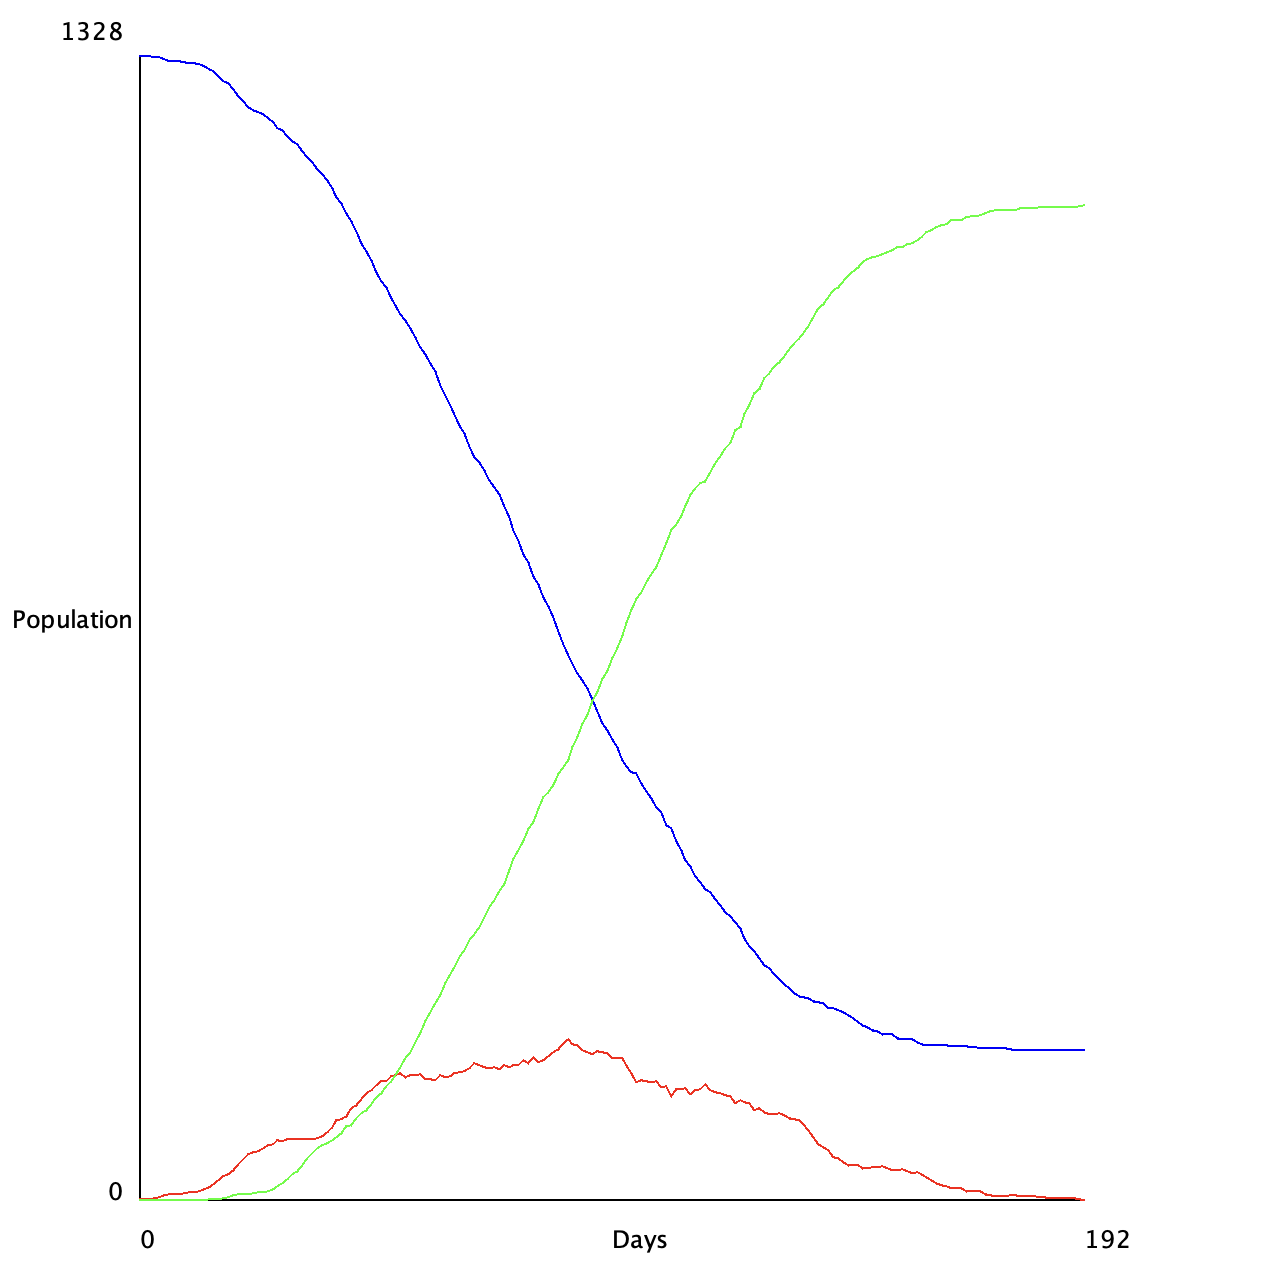
\includegraphics[width=1.25in]{Figures/SIR generated graph.png}
\caption{SIR graph relating to a simulation run}
\label{fig_sim}
\end{figure}

In the simulator, example seen in figure 7, the only available data is the graph because all of the SIR data gets compiled into a result once the simulation is closed. This is done so that multiple simulations can be recorded at once and the data that is collected across the simulations can be reported. Information like percentage of cells infected is calculated across simulations, showing how small changes in the size or algorithm may cause large impacts on infections. One thing we saw with our simulation was if you did not increase the population size as much as the size increased on the grid, infectious cells may end up isolated, preventing infections from spreading.

The model also tracks how many of the population got infected. Once the simulation is complete, the infected reach zero, we divide the total number removed by the total population. We then store this result for each simulation, and average the result. We chose to use this as a metric as it gives a better understanding as to how many of a population may catch the virus. This is incredibly important to know, especially depending on the effects of the virus.

\subsection{Multithreading Evaluation}

Our multithreading benchmarking revealed some shocking results. We found that our speedup was actually in the negatives for small simulations and only improves once the simulation is working on a large set of communities. To benchmark our parallel code, we recorded the time in nanoseconds just before the threads spin up, to just after they are destroyed and they all complete the infection step our our simulation. This time is then converted to a running average across a simulations for each day. This data allows us to track on average how much faster is this infection algorithm running in parrallel across a simulaiton.

\begin{figure}[!hbt]
\centering
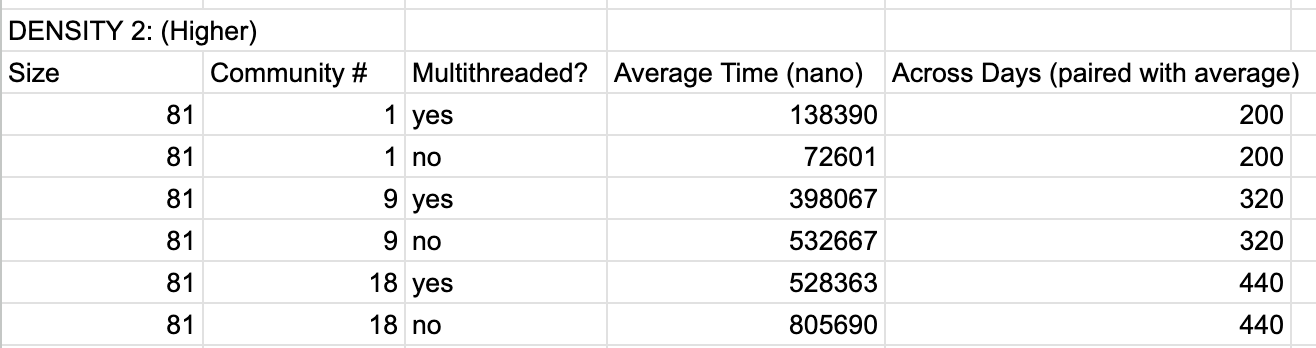
\includegraphics[width=2.5in]{Figures/High Denisty Evaluation (without extra speedup data).png}
\caption{Multithreading data across a grid size of 81x81 on different community numbers.}
\label{fig_sim}
\end{figure}

With highly populated communities, where most of the grid are members of the population, our multithreading code runs slower with a single community, but begins to run faster on larger communities. We chose to record data for single communities, 9 communities and 18 communities. These numbers were mostly arbitrary, but were chosen on how smooth the simulation was able to keep up the rendering to the actual speed of the multithreaded steps.

In figure 8, we see that the average amount of nanoseconds is greater for our parallel implementation for one community but smaller for community sizes 9 and 18. When comparing the sequential to multithreaded runs we see a 0.52x increase for one community, it is running slower when multithreaded, a 1.34x increase for communities of size 9, and a 1.52x increase for communities of size 18. This also shows that the number of communities does not appear to be a linear relationships with the amount of speedup we receive from multithreading.

Another potential problem with our speedup is likely due to cache hits. By having the algorithm run in by communities, rows, and columns, the way the algorithm traverses the graph will impact the speed. Missing out on optimizations for cache hits, and losing our program some performance on top of our threading implementation.

\begin{figure}[!hbt]
\centering
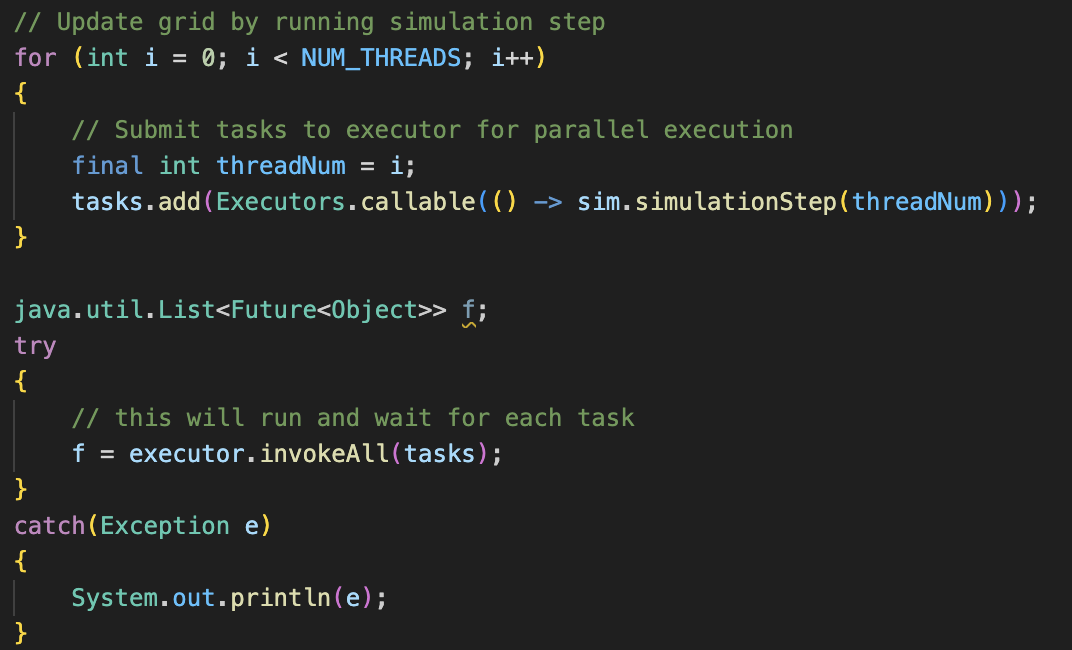
\includegraphics[width=2.5in]{Figures/multithreading set up.png}
\caption{Multithreading instantiation code}
\label{fig_sim}
\end{figure}

As we used Java as our language and were building and destroying threads for each simulation tick, the overhead of creating the threads destroyed any performance gains for small simulations, and severly limited speedup on larger simulations. This can be seen in figure 9, our multithreading code where every thread must be built and run to completion. This was a major factor for our struggle to speed up our program believe that unfortunately to resolve this multithreading problem a lot of the implementation would need to be revised or built from the ground up.


\section{Discussion}

\subsection{Implementation Challenges}

One of the biggest challenges was figuring out where to implement the multithreading. After deciding on the SIR algorithm, we found the algorithm to be too straight-forward to break apart into threads. However, we realized, because of the randomness of our implementation of the algorithm, it would make sense to run it multiple times to get an average of the epidemic results. We also decided to expand on the algorithm by adding communities to also address this challenge. This made the use of multithreading in our algorithm more clear, and also gave more value to an implementation with it.

Another challenge we encountered was implementing the SIR model itself.The original SIR model is just an equation, but coding allows for further development of it. Examples would be the randomness of where members of a community will travel, and how many other members they will encounter. Researching the SIR model only got us so far, and we had to figure out how our implementation should reflect the SIR states and interactions. 

The implementation of multiple communities in the model took a lot of innovation. The concept of communities using a grid based system was not somthing we saw in existing models. The actual implementation was more difficult than anticipated as threads were originally handling every aspect of a simulation frame. We decided to move this movement across communities and SIR collection outside of the multithreaded work, but allow the threads to do the infection step for all communities. We felt we had to make this change in particular, since separate threads are handling the different communities simultaneously, it was difficult to have cells “visit” other communities at run-time while also keeping all of the data accurate. 

Visualizing the SIR data was also a big challenge. We first decided that simple print statements would do, and we would try to add something more visually pleasing if we had the time. The grid we decided to implement was buggy at first. Trying to visualize the simulation while multiple threads were constantly changing the values caused the output to be unreliable. However, we were able to fix this, and even added a graph that may make the data easier to understand.

\subsection{Benchmarking Challenges}

While running the simulation, it was apparent that rendering the grid took much longer than it took to run each simulation step. This caused benchmarking to be difficult. To solve this problem, we separated the simulation from the frame rate by introducing a tick rate. This is a technique that allows our simulation to run as fast as possible without being bottlenecked by the rendering time. This has a drawback of not being able to render each simulation step if the tick rate is faster than the frame rate. However, this is a fine sacrifice as the rendering of the simulation is not particularly important. 

When testing different implementations of multithreading to determine which implementation would result in the largest performance gain. The current one has provided the best results. When making it apply for the variable communities, the performance gain could not outweigh the overhead since the amount of communities that would need to be running in order to possibly see an improvement would be too resource heavy which in turn would counter the performance gained. We decided to implement another instance of multithreading in both the sections of the communities and the movement of the cells. The overhead from both multithreaded operations heavily outweighed the gains that the concurrency provides. The current implementation that we have seems to be the goldilocks zone for our project.

Trying to revise the multithreading solution to prevent threads from being rebuilt and destroyed was a challenge we could not resolve with our implementation. Although we considered the grid split when deciding on our multithreading solution, our choice in language and implementation of simulation steps made it so that once we got to test our multithreading on our simulation with everything included, we were bound to having the threads run to completion, preventing them from idling for the next simulation step to occur. Because of the way Java handles threads, revising the multithreading to allow threads to idle would require us to re-implement and overhaul much of our code to support this separate implementation style.

\subsection{Future Research}

To enhance the parallelization and multithreading capabilities of the epidemic simulator, various avenues of exploration exist. Firstly, the current region-based thread assignment strategy can be modified with fine-grained parallelization techniques to exploit the available CPU cores more effectively. This entails implementing parallel loops or task-based parallelism within each region to maximize concurrency. Additionally, load balancing strategies, such as work stealing or workload-aware partitioning, can be investigated to evenly distribute the computational workload among threads, preventing any thread from idling while others are active. Asynchronous processing can also be introduced to overlap computation with her non-computational tasks, improving overall efficiency. Optimizing data sharing between threads and minimizing synchronization overhead through techniques like thread-local storage or immutable data structures may also be useful for enhancing parallelism. Furthermore, fine-tuning the thread pool configuration and exploring cache efficiency optimizations may lead to significant performance gains. Through these explorations, the parallel epidemic simulator may be optimized to fully utilize the power of parallelization and multithreading, resulting in improved efficiency and performance.

\section{Conclusion}

Our simulation successfully provides visualization and supplemental SIR data that can help users understand some of the trends and complexity that Epidemics contain. Although there were some challenges with modeling SIR as a simulation and simulation scaling, this program provides a nice visual to represent the spread of infections. One area we wish we had more time to improve is the SIR model, to track similar to existing viral data, and improvements to the simulation, making the simulator more robust.

\begin{thebibliography}{00}
\bibitem{b1} lwaw, ``Cellular-Automata-Simulator.'' https://github.com/lwaw/Cellular-Automata-Simulator. 
\bibitem{b2} L.W.A.W. gaming. ``Simulation of a viral infection on a grid,'' YouTube, Sep 19, 2020. https://www.youtube.com/watch?v=SLnWW0DG24Y (accessed Jan 31, 2024).
\bibitem{b3} M. Salathé, N. Case ``What Happens Next? COVID-19 Futures, Explained With Playable Simulations.'' https://ncase.me/covid-19/ (accessed Mar 31, 2024).
\bibitem{b4} Primer, ``Epidemic, Endemic, and Eradication Simulations.'' YouTube, May 17, 2020. https://www.youtube.com/watch?v=7OLpKqTriio (accessed Jan 31, 2024).
\bibitem{b5} 3b1b, ``sir.py.'' https://github.com/3b1b/videos/blob/master/\_2020/sir.py.
\bibitem{b6} 3Blue1Brown, ``Simulating an epidemic.'' YouTube,  Mar 27, 2020. https://www.youtube.com/watch?v=gxAaO2rsdIs (accessed Jan 31, 2024).
\bibitem{b7} Jamison, D. T. (2018). Disease control priorities. improving health and reducing poverty. World Bank Group. (accessed April 1, 2024).
\bibitem{b8} K. Simler, ``Outbreak.'' https://meltingasphalt.com. https://meltingasphalt.com/interactive/outbreak/ (accessed Apr 1, 2024). 

\end{thebibliography}
\vspace{12pt}
\color{red}
\end{document}
